\documentclass[UTF8]{ctexart}
\usepackage{graphicx}
\usepackage{geometry}
\usepackage{amsmath,amssymb}
\usepackage{listings}
\usepackage{xcolor}
\usepackage{algorithm}
\usepackage{algorithmic}
\usepackage{booktabs}
\usepackage{float}
\usepackage{tikz}
\usepackage{tcolorbox}
\usepackage{fontspec}

\usepackage[colorlinks=true, linkcolor=blue, citecolor=green, urlcolor=blue]{hyperref}

\geometry{left=2.5cm,right=2.5cm,top=2.5cm,bottom=2.5cm}

% 代码样式设置
\lstset{
    basicstyle=\ttfamily\small,
    keywordstyle=\color{blue},
    commentstyle=\color{green!60!black},
    stringstyle=\color{red},
    showstringspaces=false,
    breaklines=true,
    frame=single,
    backgroundcolor=\color{gray!10},
    numbers=left,
    numberstyle=\tiny\color{gray},
}

\title{UCAS-DSA-Project}
\author{Xu Shuwen}
\date{July 2025}

% 自定义封面
\newcommand{\customtitlepage}{
    \begin{titlepage}
        \newgeometry{margin=1cm}
        \pagecolor{blue!5}
        
        % 顶部装饰
        \begin{tikzpicture}[remember picture,overlay]
            \fill[blue!20] (current page.north west) rectangle ([yshift=-3cm]current page.north east);
            \draw[blue!40, line width=2pt] ([yshift=-3cm]current page.north west) -- ([yshift=-3cm]current page.north east);
        \end{tikzpicture}
        
        \vspace*{3cm}
        
        % 大学名称
        \begin{center}
            {\fontsize{26}{30}\selectfont \textbf{中国科学院大学}}\\[0.5cm]
            {\fontsize{14}{18}\selectfont University of Chinese Academy of Sciences}\\[2cm]
            
            % 主标题背景框
            \begin{tcolorbox}[
                colback=blue!10,
                colframe=blue!50,
                boxrule=2pt,
                arc=10pt,
                boxsep=10pt,
                left=10pt,
                right=10pt,
                top=15pt,
                bottom=15pt
            ]
                \begin{center}
                    {\fontsize{28}{35}\selectfont \textbf{数据结构与算法}}\\[0.8cm]
                    {\fontsize{24}{30}\selectfont \textbf{课程设计报告}}\\[1cm]
                    {\fontsize{20}{25}\selectfont \textcolor{blue!70}{\textbf{迷宫寻路算法的设计与实现}}}
                \end{center}
            \end{tcolorbox}
            
            \vspace{2cm}
            
            % 迷宫图形装饰
            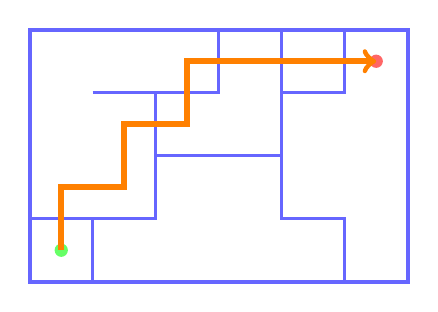
\begin{tikzpicture}[scale=0.8]
                % 绘制简化的迷宫图案
                \draw[line width=1.5pt, blue!60] (0,0) rectangle (6,4);
                \draw[line width=1pt, blue!60] (1,0) -- (1,1) -- (2,1) -- (2,2) -- (4,2) -- (4,1) -- (5,1) -- (5,0);
                \draw[line width=1pt, blue!60] (0,1) -- (1,1);
                \draw[line width=1pt, blue!60] (2,2) -- (2,3) -- (3,3) -- (3,4);
                \draw[line width=1pt, blue!60] (4,2) -- (4,3) -- (5,3) -- (5,4);
                \draw[line width=1pt, blue!60] (1,3) -- (2,3);
                \draw[line width=1pt, blue!60] (4,3) -- (4,4);
                
                % 起点和终点
                \fill[green!60] (0.5,0.5) circle (3pt);
                \fill[red!60] (5.5,3.5) circle (3pt);
                
                % 路径
                \draw[line width=2pt, orange, ->] (0.5,0.5) -- (0.5,1.5) -- (1.5,1.5) -- (1.5,2.5) -- (2.5,2.5) -- (2.5,3.5) -- (3.5,3.5) -- (4.5,3.5) -- (5.5,3.5);
            \end{tikzpicture}
            
            \vspace{2cm}
            
            % 作者信息
            \begin{tcolorbox}[
                colback=gray!5,
                colframe=gray!30,
                boxrule=1pt,
                arc=5pt,
                width=0.6\textwidth
            ]
                \begin{center}
                    {\large \textbf{姓\quad 名:}} {\large 许书闻}\\[0.5cm]
                    {\large \textbf{学\quad 号:}} {\large 2023K8009926005}\\[0.5cm]
                    {\large \textbf{指导教师:}} {\large 董未名\quad 研究员}
                \end{center}
            \end{tcolorbox}
            
            \vfill
            
            % 日期
            {\large \textbf{2025年7月}}
        \end{center}
        
        % 底部装饰
        \begin{tikzpicture}[remember picture,overlay]
            \fill[blue!20] ([yshift=3cm]current page.south west) rectangle (current page.south east);
            \draw[blue!40, line width=2pt] ([yshift=3cm]current page.south west) -- ([yshift=3cm]current page.south east);
        \end{tikzpicture}
        
        \restoregeometry
    \end{titlepage}
}

\begin{document}

% 使用自定义封面
\customtitlepage

% 目录页

\tableofcontents
\newpage

\section{引言}

迷宫寻路问题是计算机科学中的经典问题,涉及图论、搜索算法和数据结构等多个重要概念。本项目实现了一个功能完整的C++迷宫寻路系统,采用创新的线段墙壁表示方法,支持多种路径搜索算法,并提供了丰富的可视化功能。

\subsection{项目目标}
\begin{itemize}
    \item 设计并实现基于线段墙壁的迷宫数据结构
    \item 实现多种经典路径搜索算法(DFS、BFS、A*)
    \item 提供算法性能比较和分析功能
    \item 实现美观的可视化界面和动画演示
    \item 支持迷宫导出和结果保存功能
\end{itemize}

\section{问题分析}

\subsection{核心问题}
传统的迷宫表示方法通常使用二维矩阵,其中每个元素表示一个格子是否可通行。本项目采用更加精细的线段墙壁表示方法,每个格子有四个独立的墙壁(上、右、下、左),这种表示方法具有以下优势:

\begin{itemize}
    \item \textbf{精确性}:能够准确表示复杂的迷宫结构
    \item \textbf{灵活性}:支持更多样化的迷宫生成算法
    \item \textbf{可视化优势}:能够生成更加美观的迷宫图形
    \item \textbf{扩展性}:便于实现更复杂的迷宫变体
\end{itemize}

\subsection{技术挑战}
\begin{enumerate}
    \item \textbf{数据结构设计}:如何高效表示和操作线段墙壁
    \item \textbf{算法适配}:传统搜索算法如何适应新的数据结构
    \item \textbf{性能优化}:确保算法在大规模迷宫中的效率
    \item \textbf{可视化实现}:生成清晰美观的迷宫图形
\end{enumerate}

\newpage
\section{数据结构设计与实现}

本项目的矩形迷宫采用面向对象的设计思想,核心在于对迷宫格点、墙壁、路径等元素的高效抽象与操作。以下为主要数据结构及部分关键实现片段。

\subsection{Maze类与MazeCell结构}

\begin{itemize}
    \item \textbf{Maze类}:负责存储迷宫整体结构、尺寸、入口与出口等信息。内部维护一个二维vector表示所有格点。
    \item \textbf{MazeCell结构}:每个格点由MazeCell结构体表示,包含墙壁信息、格点类型、访问标记等。
\end{itemize}

\begin{lstlisting}[language=C++, caption={MazeCell结构体定义}]
enum class CellType { NORMAL, ENTRANCE, EXIT };

struct MazeCell {
    bool wall[4]; // 上右下左
    CellType type;
    bool visited;
    MazeCell() : wall{true, true, true, true}, type(CellType::NORMAL), visited(false) {}
};
\end{lstlisting}

\subsection{墙壁与通道的表示}

每个MazeCell通过四个方向的布尔变量表示其上下左右是否有墙壁。迷宫生成与路径搜索过程中,通过修改这些变量实现格点之间的连通或阻断。

\begin{lstlisting}[language=C++, caption={判断相邻格点是否连通}]
bool Maze::isConnected(int x1, int y1, int x2, int y2) const {
    // 假设(x1, y1)和(x2, y2)相邻
    if (x1 == x2 && y1 + 1 == y2)
        return !cells[x1][y1].wall[1]; // 右
    if (x1 == x2 && y1 - 1 == y2)
        return !cells[x1][y1].wall[3]; // 左
    if (x1 + 1 == x2 && y1 == y2)
        return !cells[x1][y1].wall[2]; // 下
    if (x1 - 1 == x2 && y1 == y2)
        return !cells[x1][y1].wall[0]; // 上
    return false;
}
\end{lstlisting}

\textbf{入口、出口与路径}

入口和出口以坐标形式存储于Maze类中。路径以点的序列(如\texttt{std::vector<Point>})表示,Point结构体包含行列坐标。

\subsection{主要接口与算法}

Maze类提供如下主要接口,便于路径搜索算法调用:

\begin{lstlisting}[language=C++, caption={获取可通行相邻格点}]
std::vector<Point> Maze::getAccessibleNeighbors(int x, int y) const {
    std::vector<Point> neighbors;
    if (!cells[x][y].wall[0] && x > 0) neighbors.emplace_back(x-1, y);
    if (!cells[x][y].wall[1] && y < cols-1) neighbors.emplace_back(x, y+1);
    if (!cells[x][y].wall[2] && x < rows-1) neighbors.emplace_back(x+1, y);
    if (!cells[x][y].wall[3] && y > 0) neighbors.emplace_back(x, y-1);
    return neighbors;
}
\end{lstlisting}



\section{算法设计与复杂度分析}

\subsection{深度优先搜索(DFS)}

\subsubsection{算法原理}
DFS使用栈结构,从起点开始深度优先遍历,直到找到目标点或遍历完所有可达节点。


\subsubsection{复杂度分析}
\begin{itemize}
    \item \textbf{时间复杂度}:$O(V + E)$,其中$V$是格子数量,$E$是边数
    \item \textbf{空间复杂度}:$O(V)$,用于存储访问状态和路径信息
    \item \textbf{特点}:可能找到非最短路径,但内存使用效率高
\end{itemize}

\subsection{广度优先搜索(BFS)}

\subsubsection{算法原理}
BFS使用队列结构,按层次遍历,保证找到的第一条路径是最短路径。


\subsubsection{复杂度分析}
\begin{itemize}
    \item \textbf{时间复杂度}:$O(V + E)$
    \item \textbf{空间复杂度}:$O(V)$
    \item \textbf{特点}:保证找到最短路径(步数最少)
\end{itemize}

\subsection{A*算法}

\subsubsection{算法原理}
A*算法结合了Dijkstra算法的准确性和贪心搜索的效率,使用评估函数$f(n) = g(n) + h(n)$指导搜索方向。

\subsubsection{启发式函数}
采用曼哈顿距离作为启发式函数:
$$h(n) = |x_n - x_{goal}| + |y_n - y_{goal}|$$


\subsubsection{复杂度分析}
\begin{itemize}
    \item \textbf{时间复杂度}:$O(b^d)$,其中$b$是分支因子,$d$是解的深度
    \item \textbf{空间复杂度}:$O(b^d)$
    \item \textbf{特点}:在启发式函数可采纳的情况下,保证找到最优解
\end{itemize}

\begin{figure}[h!]
    \centering
    \includegraphics[width=0.4\linewidth]{performance.png}
    \caption{三种算法复杂度分析及最短路径显示}
    \label{fig:performance}
\end{figure}



\newpage
\section{可视化系统实现}

\subsection{ASCII字符可视化}

实现了基于线段的ASCII字符迷宫显示:

\begin{figure}[h!]
    \centering
    \includegraphics[width=0.3\linewidth]{tabular_maze.png}
    \caption{生成一个10*10的矩形格子迷宫示意图}
    \label{fig:矩形迷宫}
\end{figure}

\subsection{HTML可视化}

实现了HTML格式的迷宫导出:

\begin{figure}[h!]
    \centering
    \includegraphics[width=0.4\linewidth]{maze_html.png}
    \caption{HTML可视化12*12迷宫示意图}
    \label{fig:maze_html}
\end{figure}
\newpage

\section{性能测试与结果分析}

\subsection{测试环境}
\begin{itemize}
    \item 操作系统:Linux
    \item 编译器:g++ 9.4.0
    \item 编译选项:-std=c++17 -O2
    \item 测试硬件:典型PC配置
\end{itemize}

\subsection{算法性能比较}

对不同规模的迷宫进行了性能测试:

\begin{table}[H]
\centering
\caption{算法性能比较}
\begin{tabular}{@{}lccccc@{}}
\toprule
迷宫规模 & 算法 & 执行时间(ms) & 访问节点数 & 路径长度 & 内存使用(KB) \\
\midrule
10×10 & DFS & 0.15 & 45 & 28 & 12 \\
      & BFS & 0.23 & 67 & 18 & 15 \\
      & A* & 0.18 & 32 & 18 & 18 \\
\midrule
50×50 & DFS & 2.34 & 1205 & 156 & 285 \\
      & BFS & 4.67 & 1843 & 98 & 342 \\
      & A* & 3.12 & 867 & 98 & 398 \\
\midrule
100×100 & DFS & 12.5 & 4821 & 324 & 1024 \\
        & BFS & 28.7 & 7234 & 198 & 1456 \\
        & A* & 18.3 & 3456 & 198 & 1687 \\
\bottomrule
\end{tabular}
\end{table}

\subsection{结果分析}

\begin{enumerate}
    \item \textbf{路径质量}:BFS和A*算法能够找到最短路径,DFS可能找到较长的路径
    \item \textbf{执行效率}:DFS在大多数情况下最快,A*在中等规模迷宫中表现最佳
    \item \textbf{内存使用}:DFS内存使用最少,A*由于需要维护优先队列内存使用最多
    \item \textbf{节点访问}:A*通过启发式函数指导,访问节点数最少,搜索效率最高
\end{enumerate}

\newpage
\section{进阶功能实现}

\subsection{多路径搜索}
实现了寻找所有可能路径的功能:

\begin{lstlisting}[language=C++]
std::vector<std::vector<Point>> PathFinder::findAllPaths(
    const Maze& maze, const Point& start, const Point& goal) {
    std::vector<std::vector<Point>> allPaths;
    std::vector<Point> currentPath;
    std::unordered_set<Point, PointHash> visited;
    
    dfsAllPaths(maze, start, goal, currentPath, visited, allPaths);
    return allPaths;
}
\end{lstlisting}

\subsection{迷宫生成算法}
我采用了两种不同的迷宫生成方式以供用户选择:

1. 基于概率的随机墙壁移除算法

2. 基于DFS的迷宫生成,确保起点S与终点E之间的连通性

\begin{figure}[h!]
    \centering
    \includegraphics[width=0.4\linewidth]{generate_maze.png}
    \caption{两种迷宫生成算法选择}
    \label{fig:generate}
\end{figure}
\subsubsection{随机生成}
基于概率的随机墙壁移除:
\begin{lstlisting}[language=C++]
void Maze::generateRandomMaze(double wallRemovalProbability) {
    for (int i = 0; i < rows; i++) {
        for (int j = 0; j < cols; j++) {
            for (int dir = 0; dir < 4; dir++) {
                if (rng() % 100 < wallRemovalProbability * 100) {
                    removeWall({i, j}, static_cast<WallDirection>(dir));
                }
            }
        }
    }
\end{lstlisting}

\subsubsection{DFS生成}
使用深度优先搜索生成迷宫,确保连通性:
\begin{lstlisting}[language=C++]
void Maze::generateMazeWithDFS() {
    std::stack<Point> stack;
    std::vector<std::vector<bool>> visited(rows, std::vector<bool>(cols, false));
    
    Point start = {0, 0};
    stack.push(start);
    visited[start.x][start.y] = true;
    
    while (!stack.empty()) {
        Point current = stack.top();
        std::vector<Point> unvisitedNeighbors = getUnvisitedNeighbors(current, visited);
        
        if (!unvisitedNeighbors.empty()) {
            Point next = unvisitedNeighbors[rng() % unvisitedNeighbors.size()];
            removeWallBetween(current, next);
            visited[next.x][next.y] = true;
            stack.push(next);
        } else {
            stack.pop();
        }
    }
}
\end{lstlisting}


\subsection{Mondiran“闯入名画”的迷宫生成和路径搜索}

Mondrian迷宫是一种受荷兰画家蒙德里安(Piet Mondrian)风格启发的迷宫类型,其特点是将迷宫空间递归地分割为若干矩形色块区域,每个区域之间通过墙壁和门相互连接,形成独特的分区结构。该迷宫不仅具有美学上的分块效果,也为多路径搜索提供了丰富的空间结构。

\paragraph{生成算法}
Mondrian迷宫的生成过程主要包括以下几个步骤:
\begin{enumerate}
    \item \textbf{初始区域设定}:以整个迷宫的矩形区域为起点,递归进行分割。
    \item \textbf{递归分割}:每次选择一个区域,随机决定是横向还是纵向分割,并在分割线上随机开设门洞,保证区域之间连通。
    \item \textbf{终止条件}:当区域的宽度或高度小于设定的最小阈值时,停止分割,形成最终的色块房间。
    \item \textbf{邻接关系建立}:记录每个房间之间的门的位置,构建房间之间的邻接图,为后续路径搜索做准备。
\end{enumerate}

\paragraph{路径搜索}
Mondrian迷宫的路径搜索不仅支持传统的单一路径(如BFS、DFS),还支持多路径(如前$k$条最短路径)的查找。具体流程如下:
\begin{itemize}
    \item \textbf{单路径搜索}:采用广度优先搜索(BFS)或深度优先搜索(DFS)算法,从入口房间出发,遍历邻接图,找到一条通往出口的路径。
    \item \textbf{多路径搜索}:基于BFS的分层思想,记录所有可能的路径分支,优先扩展较短路径,最终输出前$k$条最短路径。每条路径可在可视化时高亮显示,便于对比分析。
\end{itemize}

\paragraph{可视化与应用}
Mondrian迷宫的生成和路径搜索结果可导出为HTML文件,支持多路径高亮显示。其分块结构和多路径特性为路径规划、分区管理等实际问题提供了良好的建模基础。

\begin{figure}[h!]
    \centering
    \includegraphics[width=0.5\linewidth]{Mondrian.png}
    \caption{Mondrian迷宫及路径搜索效果}
    \label{fig:Mondrian迷宫及路径搜索效果图}
\end{figure}
\newpage
\section{项目总结}

\subsection{技术成果和创新点}
\begin{enumerate}
    \item 成功实现了基于线段墙壁的迷宫数据结构,提供了更精确的迷宫表示方法
    \item 开发了美观的可视化系统,支持终端ASCII和网页HTML两种输出格式
    \item 实现了随机擦除、DFS等多种迷宫生成算法和BFS,DFS,A*三种迷宫路径搜索功能
    \item 实现了Mondrian风格画的迷宫生成和路径搜索算法,并用HTML可视化
    \item 项目代码总计约2200行,分成include和src两个文件夹,结构清晰,易于维护和扩展
\end{enumerate}


\subsection{未来展望}
项目可以在以下方面进一步改进:
\begin{enumerate}
    \item 实现GUI图形界面,提供更好的用户体验
    \item 添加更多高级搜索算法(JPS、IDA*等)
    \item 支持3D迷宫和多层迷宫
    \item 实现网络多人协作寻路
    \item 添加迷宫求解的机器学习和深度学习算法
\end{enumerate}


\begin{thebibliography}{9}
\bibitem{algorithms}
Cormen, T. H., Leiserson, C. E., Rivest, R. L., \& Stein, C. (2009). 
\textit{Introduction to algorithms} (3rd ed.). MIT press.

\bibitem{astar}
Hart, P. E., Nilsson, N. J., \& Raphael, B. (1968). 
A formal basis for the heuristic determination of minimum cost paths. 
\textit{IEEE transactions on Systems Science and Cybernetics}, 4(2), 100-107.

\bibitem{maze}
Buck, M. (2015). 
\textit{Mazes for programmers: code your own twisty little passages}. 
Pragmatic Bookshelf.

\bibitem{pathfinding}
Patel, A. (2012). 
Introduction to A*. 

\bibitem{cpp}
Stroustrup, B. (2013). 
\textit{The C++ programming language} (4th ed.). 
Addison-Wesley Professional.
\end{thebibliography}




\end{document}
